\chapter{序論}

\section{はじめに}
1953年、James WatsonとFrancis Crickは、遺伝情報の実体は4種類のデオキリボ核酸が相補的に水素結合した二重らせん構造であること鮮やかに示した。5年後の1958年、Clickは"Ideas for protein synthesis"において、遺伝情報はDNA-RNA-タンパクへと一方向性を持って伝達されるという分子生物学におけるセントラルドグマ (中心原理)を提唱した (図\ref{fig:crick_idea})。1960年代から70年代には、Maurice WilkinsやSydney Brennerなど多くの研究者により、コドンの発見と遺伝暗号が解読されると、塩基配列がアミノ酸を表現する基本原則が明らかとなった。黎明期における分子生物学は、物理学者が多く参入した経緯も相まって、分子のことばで生命の持つ普遍的性質の理解を標榜する学問として誕生し、熾烈な競争の下に急速な進展を遂げた。
\begin{figure}[htbp]
	\begin{center}
		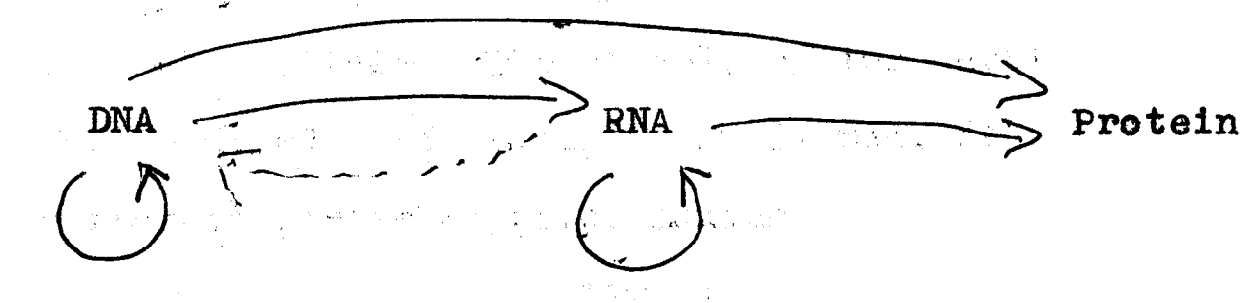
\includegraphics[width=14cm]{crick_idea.png}
	\end{center}
	\caption{\textit{"Ideas on Protein Synthesis"}, (Oct, 1956)}
	\label{fig:crick_idea}
\end{figure}
\par
今日までの分子生物学研究の発展は、生物に普遍的だと考えられてきた数々の性質や分子機序からの「逸脱」や「例外」をも同時に明らかにしてきた。1970年、Howard TeminおよびDavid Baltimoreは一本鎖RNAを鋳型として、相補的なDNAを合成する逆転写酵素を発見した。この発見は、セントラルドグマから逸脱し、RNAからDNAへも遺伝情報は伝達しうることを示した画期的な発見であった。その後も、真核生物における遺伝子はスプライシング機構によってイントロンが切り出され複数のエクソンから構成されること、転写直後の新生RNAは3'末端にポリアデニル化、5'末端にはキャップ構造が付加されて成熟すること、線虫からはコドンが異なるアミノ酸をコードする例外が発見されるなど、セントラルドグマの概念もまた時代とともに拡張されてきた。このことは、本質的には、生命が逸脱や例外を含む多様性を担保する存在であることに他ならない。生命の持つ普遍的な性質の理解を目指した分子生物学において、逸脱や例外といった個別的な生命現象をその対象することが逆説的には、生命の理解へと接続される重要なアプローチの一つだと私は考えている。
%\par
%転写はゲノム上にコードされた遺伝情報をRNAへ正確にコピーする機構を指す。転写は核内で起こる生化学反応であり、RNAポリメラーゼよって触媒される。転写されたpre-mRNAはスプライシング、ポリアデニル化と5'キャップ付加を受けて成熟した後に、核膜孔を通して細胞質へ輸送される、というのが転写機構の大まかな素描である。ヒトゲノムの解読前、遺伝子数はおよそ10万個だと見積もられていたが、2004年の完了宣言では2.5万個程度に大きく下方修正され、直感的な生命の複雑性と遺伝子数には直接の相関関係が見られないことは今日に繰り返すまでもない。
\par
真核生物の多様で複雑なシステムは、セントラルドグマからの逸脱の他に塩基やタンパク質への修飾が生命活動に不可欠であることは、現在の分子生物学においては前提となっている。細胞の内外の情報伝達には、キナーゼによるタンパク質のカスケード的なリン酸化反応が用いられ、リン酸化された分子が核内に移行し転写因子の活性を調節することで遺伝子発現の状態と量が制御される。核内において、ヒストンはアセチル基やメチル基による化学修飾を受け、染色体構造の変化を伴った遺伝子発現調節や細胞の分化状態が決定されるなど、修飾の持つ生体内機序の制御例は枚挙にいとまがない。真核生物においては有限個の遺伝子にその種数を規定されながらも、転写および翻訳機構からの逸脱や修飾によって巧妙な多様かつ複雑な機構が実現されている。
\par
本研究が対象としているのはRNA editing (RNA編集)という転写後修飾 (post-transcriptional modification)の一種である。RNA 
editingは、DNAにコードされた遺伝情報がRNAポリメラーゼにより転写された直後、RNAが別のヌクレオシドに置換される現象を指す。RNA editingを受けた転写物は、元来の遺伝情報とは異なった配列情報を持つこととなり、こういった意図的な修飾は、DNAから正確なコピーとしてのRNAを合成するという転写機構からの明らかな逸脱と考えることができる。興味深いことにヒトやマウス、ショウジョウバエといった高等真核生物においては、特定の遺伝子領域内へRNA editingを起こし、タンパク活性の変化や機能の調節に積極的に利用されているとの報告が蓄積している。また、ここ数年の超並列シーケンシング (High-throughput sequencing, HTSeq)によるトランスクリプトームの網羅的かつ定量的な計測は、非翻訳RNAやイントロン領域などこれまで研究対象とされなかった転写領域におけるRNA editingに光をあてており、非翻訳領域におけるRNA editingの生物学的な意義には、今日大きな注目が集まっている。しかしながら、超並列シーケンサーを用いた情報学的なRNA editingサイトの検出や解析は、ここ数年に立ち上がった新しい領域であることから、一度の実験で得られる膨大なシーケンシングデータから精度よくeditingサイトを同定する手法や機能解析には、確立された手法は未だ登場していない状況にある。
\par
本論文は、RNA editing研究に関する大きく2つの内容を取り扱う。一つは、超並列シーケンシングデータを用いたRNA editingサイトの検出を目的としたソフトウェア・パッケージの開発である。RNA editingサイトの検出手法を実装し、検出したサイトの精度を検証できるソフトウェア・パッケージの開発を行った。二つは、ヨコヅナクマムシのシーケンスデータからeditingサイトを検出し、その情報学的解析を行った研究である。序論では、既往の研究により明らかにされたRNA editingの生理学的な機能、超並列シーケンサーを用いたRNA editing研究の現状について概観する。第2章および3章では、既存の検出手法について性能評価を行い、高精度かつ高速な新規RNA editingサイトの検出手法の開発を行った結果を議論する。第4章では、開発した手法をヨコヅナクマムシへ適用し、RNA editingと極限環境耐性との関係性についての情報学的解析を行った。本研究は、大量のRNA-seqデータを用いたRNA editingサイトの簡便な検出を可能にし、真核生物における転写後修飾とその制御機能の更なる解明に貢献するこを期待するものである。

\newpage

\section{真核生物におけるRNA editingとADARの役割}
\subsection{A-to-I editingの多様な作用様式}
RNA editingは転写物への一塩基修飾を指し、鞭毛虫のミトコンドリアから初めて発見された。真核生物では、ADAR (adenosine deaminase acting on RNA)によるアデニン(A)からイノシン(I)へ修飾されるA-to-I editingの他に、APOBECによるシトシン(C)からウラシル(U)への修飾がこれまで報告されている。APOBECのターゲットとなる遺伝子は非常に少なく、ヒトではAPOBとNF1遺伝子のみが知られている。
植物においては主にシロイヌナズナにおけるT-to-C editing、ヒトやマウス、ショウジョウバエなど高等真核生物においてはA-to-I editingが優勢を占めることが多くの研究から明らかになっている。
\par
高等真核生物においては、アミノ酸配列の変化を伴うA-to-I editingの報告例は非コード領域におけるeditingに対して著しく少なく、非翻訳領域 (Untranslated regions, UTRs)やAlu配列といったイントロン内のレトロトランスポゾン領域におけるA-to-I editingが優勢を占めるという特徴が近年、明らかにされてきた。加えて、miRNAやRNAi (RNA interference)経路とのクロストークを介したグローバルな遺伝子発現制御との関係性などが指摘されていることから、真核生物におけるA-to-I editingを理解するためには、非翻訳RNA (non-coding RNA)におけるA-to-I editingを研究することが重要であると言える。すなわち、真核生物におけるRNA editingの理解には、従来想定されてきたようなアミノ酸置換を伴ったコード領域内へのeditingのみならず、非コード翻訳領域におけるeditingを解析し、その意味を理解することの重要性を示していると考える。超並列シーケンサーによる情報学的解析は、こういった非翻訳RNAへのeditingの存在を明らかにしてきた。
\par
本章では、RNA editing研究に関する最新の研究成果を含めて分野を概観すると同時に、大規模なシーケンシングデータを使った情報学的なA-to-I editigサイトの検出手法の発展を概観する。それを受けて、今後のediting研究の進むであろう一つの方向性を示すことができればと考える。

\subsection{ADARによるグアノシンからイノシンへの塩基修飾}
ADARは、二本鎖RNA結合タンパクの一種として知られ、二本鎖RNAと選択的に結合し、アデノシン (Adenosine)からイノシン (Inosine)への加水分解的な脱アミノ化反応を触媒する。イノシンへと置換されたヌクレオシドは、転写機構においてグアノシンとして認識される。ADARによる修飾をA-to-I editingと呼び、修飾後のグアノシンに着目した場合は、A-to-G editingとも表記するが本質的には同一である。
\par
A-to-I editingは、AからGへの一塩基置換とであるため、非同義置換によるアミノ酸の変異や終止コドンが置換され転写物が伸長するリードスルー、イントロン-エクソン境界におけるsplice siteへのediitngによるsplice siteの新生および欠失などの機能がこれまでに報告されている。図\ref{fig:Chemical_reaction}にA-to-I editingの脱アミノ化による塩基修飾反応の模式図を示す。

\begin{figure}[!htbp]
	\begin{center}
		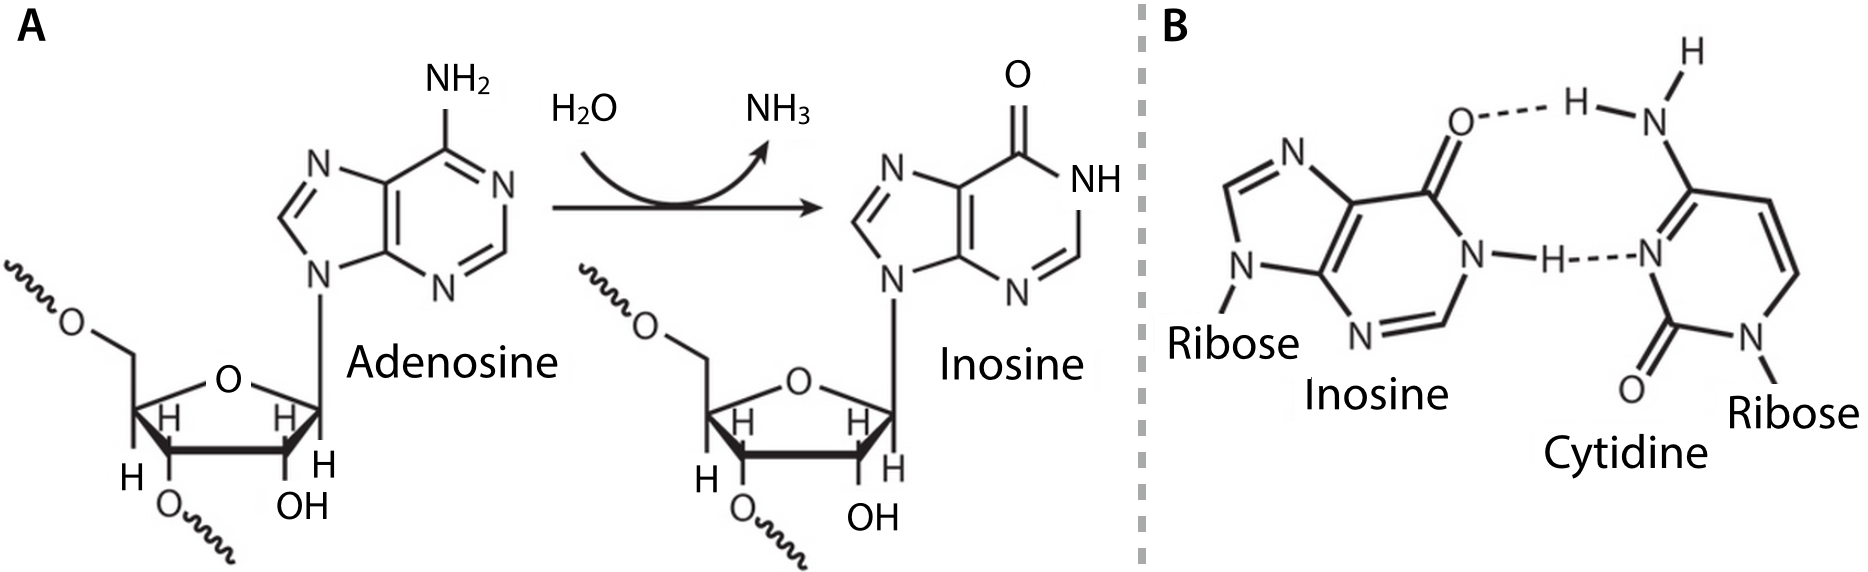
\includegraphics[width=11cm]{Adenosine-inosine.png}
	\end{center}
	\caption{ADARの生化学的な作用機序}
	\begin{flushleft}
		\small{ADARによるアデノシンからイノシンへの化学修飾が触媒される様子を示す。アデノシンはADARによる脱アミノ化反応によってイノシンへの一塩基修飾を受ける。イノシンへの修飾は同時に標的となった二本鎖RNAの二次構造を変化させる。}
	\end{flushleft}
	\label{fig:Chemical_reaction}
\end{figure}

\subsection{二本鎖RNAの二次構造と修飾塩基の選択性}
ADARによるA-to-I editingは、イノシンへ修飾されるポジションに高い選択性のある場合と、選択性が低くRNAへランダムに置換する2つのタイプに分類される。位置選択性の高いeditingは、20bp程度の短い二本鎖RNAを形成しADARのターゲットとなるのに対し、ランダムにeditingされる非選択的なeditigサイトは、二本鎖RNAは100bp以上であることが多く、非選択的なeditingは、最大でも50\%程度がイノシンへと修飾される傾向が見られることが報告されている。これまでの研究から、特定のアデノシンのみを選択的にeditingするためには、二本鎖RNAの形成する特異的に二次構造が重要であることが明らかとなっている。
\par
古くからA-to-I editingの研究対象となっているGuanosine receptor-2 (GluR2)やSerotonin receptor-2C (5-HTR)は、editingの入る位置に高い特異性を示し、特定のアデノシンのみが選択的にグアノシンへと置換される。このような位置特異的なA-to-I editingにおいては、隣接するエクソン-イントロン境界における相補的な配列、ECS (Editing-site complamentary sequence)およびその二次構造の形成が不可欠であることが知られている。
\par
Glutamine receptor (GluR)においては、editingサイト毎にADAR1またはADAR2のどちらか一方に優先的にeditingされることが知られており、位置毎におけるADARの選択性は、ADARの持つdsRBDの数とドメイン間の配列長の相違がADARと二本鎖RNAとの相互作用を変化させることに起因するとの報告がある。ヒトB細胞において、siRNAによるAdar1およびAdar2のノックダウンを別々に行った解析では、同定されたA-to-I editingのうち、20\%程度がAdar1およびAdar2の共通したターゲットとなっていることが報告されている。また、Adar1のみをサイレンシングした場合、A-to-I editingサイトの総数は1/3程度に減少することから、ヒトB細胞においてはAdar1によるA-to-I editingが優勢的であると考えられる。図\ref{fig:ADAR}に二本鎖RNAに結合するADARとそのサイトを示した。
\begin{figure}[!htbp]
	\begin{center}
		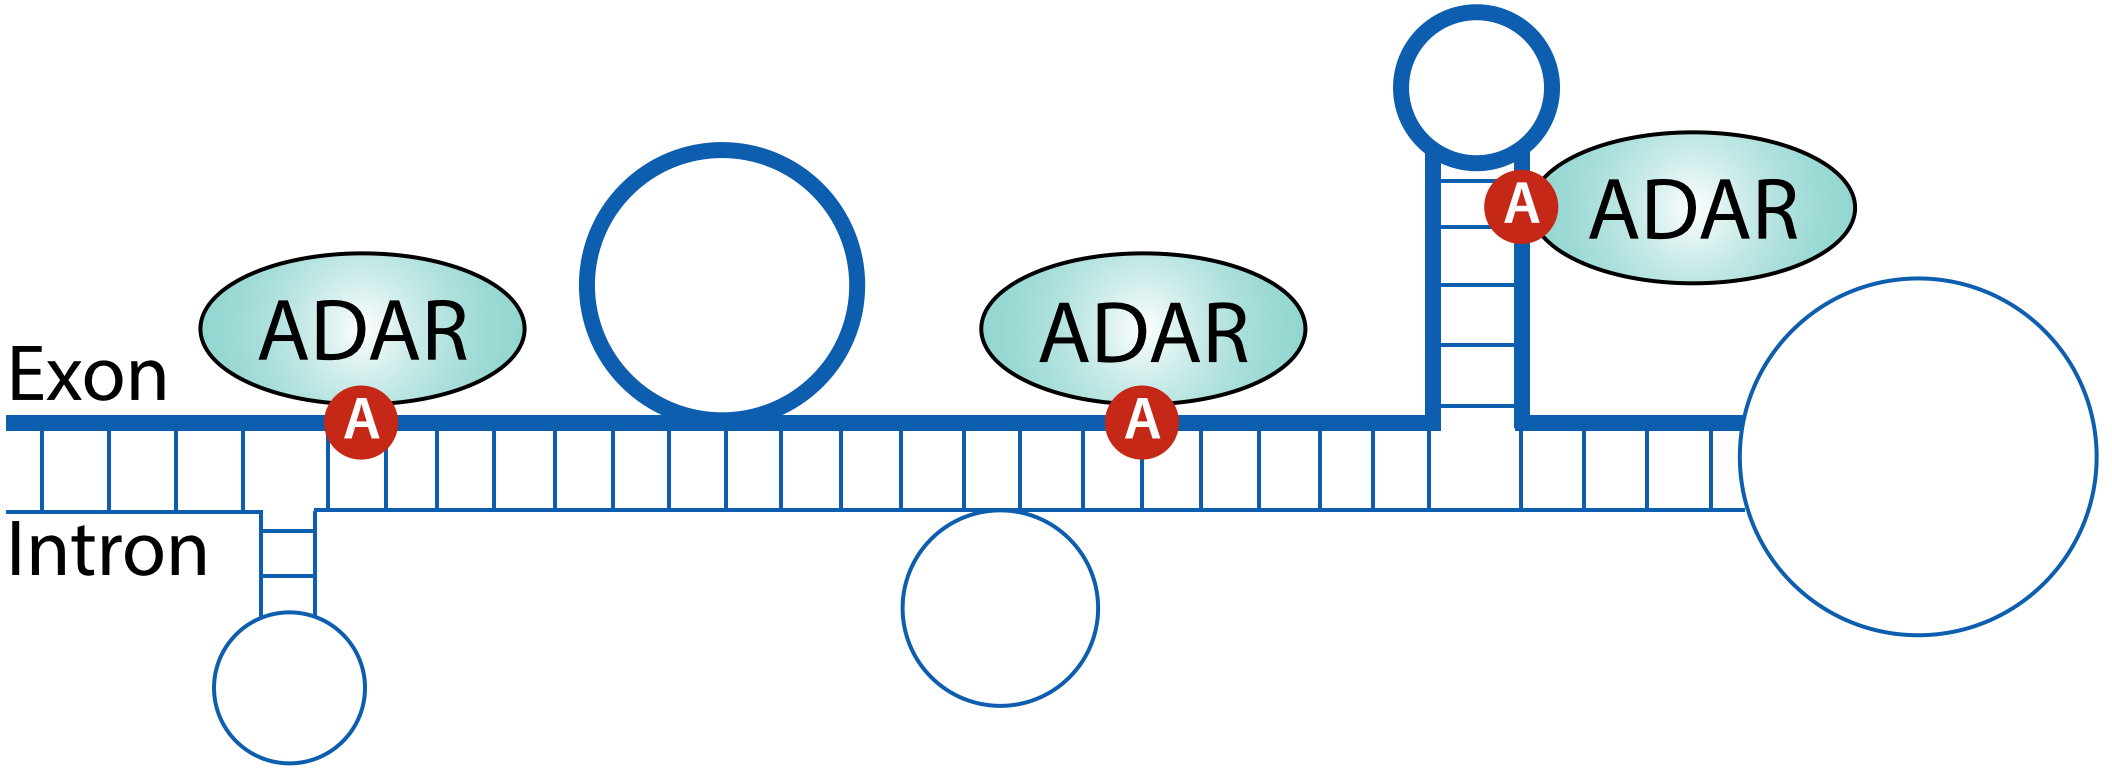
\includegraphics[width=14cm]{ADAR.png}
	\end{center}
	\caption{ADARによるA-to-I editingの模式図}
	\begin{flushleft}
		\small{ADARは二次構造を形成した二本鎖RNAへ特異的に結合し、アデノシンからイノシンへの塩基置換を触媒する。多くの転写物は複数のeditingサイトを持つことが知られる。エクソン領域(太線)に隣接するイントロン領域 (細線)の間に二次構造が形成され、3箇所にeditingが起きている様子を表す。}
	\end{flushleft}
	\label{fig:ADAR}
\end{figure}

\subsection{\textit{Adar}遺伝子の欠損による生理学的な影響}
生体内における\textit{Adar}の発現が生理学的に重要な役割を持つことは、ヒトやマウス、線虫などの変異株や遺伝子サイレンシングを用いた実験により明らかにされてきた。ショウジョウバエにおいては、\textit{Adar1}の欠損により、協調的な運動行動の欠損や加齢依存的な神経変性が報告され、線虫においては\textit{Adar1}および\textit{Adar2}のホモ変異体は、走化性が欠損することが報告されている。マウスにおける\textit{Adar1}および\textit{Adar2}はともに致死性を示す。\textit{Adar1}の変異体では初期発生段階において赤血球新生における異常によるアポトーシスが原因で致死の表現型を示し、\textit{Adar2}の欠損は、生後20日以内にけいれん重積により死に至る。この原因は、詳細は後述するが、グルタミン酸受容体におけるediting不全だとされている。
ヒトにおいては、ADARによるediting不全に起因した疾患が報告されており、\textit{Adar1}のホモ変異体は、遺伝性対側性色素異常症を引き起こす他、グルタミン酸受容体における不完全なeditingは、筋萎縮性側索硬化症の原因となることが明らかとなっている。また、未編集のセトロニン受容体が精神疾患の原因となることが指摘されている。

\subsection{ADARファミリーのドメイン構造}
図\ref{fig:adar_domain}にADARの持つ機能ドメイン構造を示す。ADARはアデノシンからイノシンへの塩基修飾を触媒するdeaminaseドメインと二本鎖RNAに結合するdsRBD (Double-strand RNA binding domain)の2つの機能ドメインをヒト、マウス、線虫、ショウジョウバエは共通して有する。dsRBDは65残基程度の長さの中にα-β-β-β-αという特徴的なドメイン構造を持ち、直接的に二本鎖RNAと接触するためA-to-I editingに必須の機能ドメインの一つである。ヒトのADAR1においては、Z-DNA-bindingドメインを1つから2つ有しているが、これはADARのターゲットとなる転写物、特にsiRNAなど短鎖の二本鎖RNAとの結合における親和性を高めるためだと考えられている。また、ヒトのADAR3のみに特徴的にアルギニンリッチな一本鎖RNA結合ドメインのR-domainを持つが、この生物学的な意義については明らかにされていない。ヒトの2つのADAR1、L型とS型はスプライシングアイソフォームとして知られ、それぞれ異なるプロモーターから転写されることが分かっている。

\begin{figure}[!htbp]
	\begin{center}
		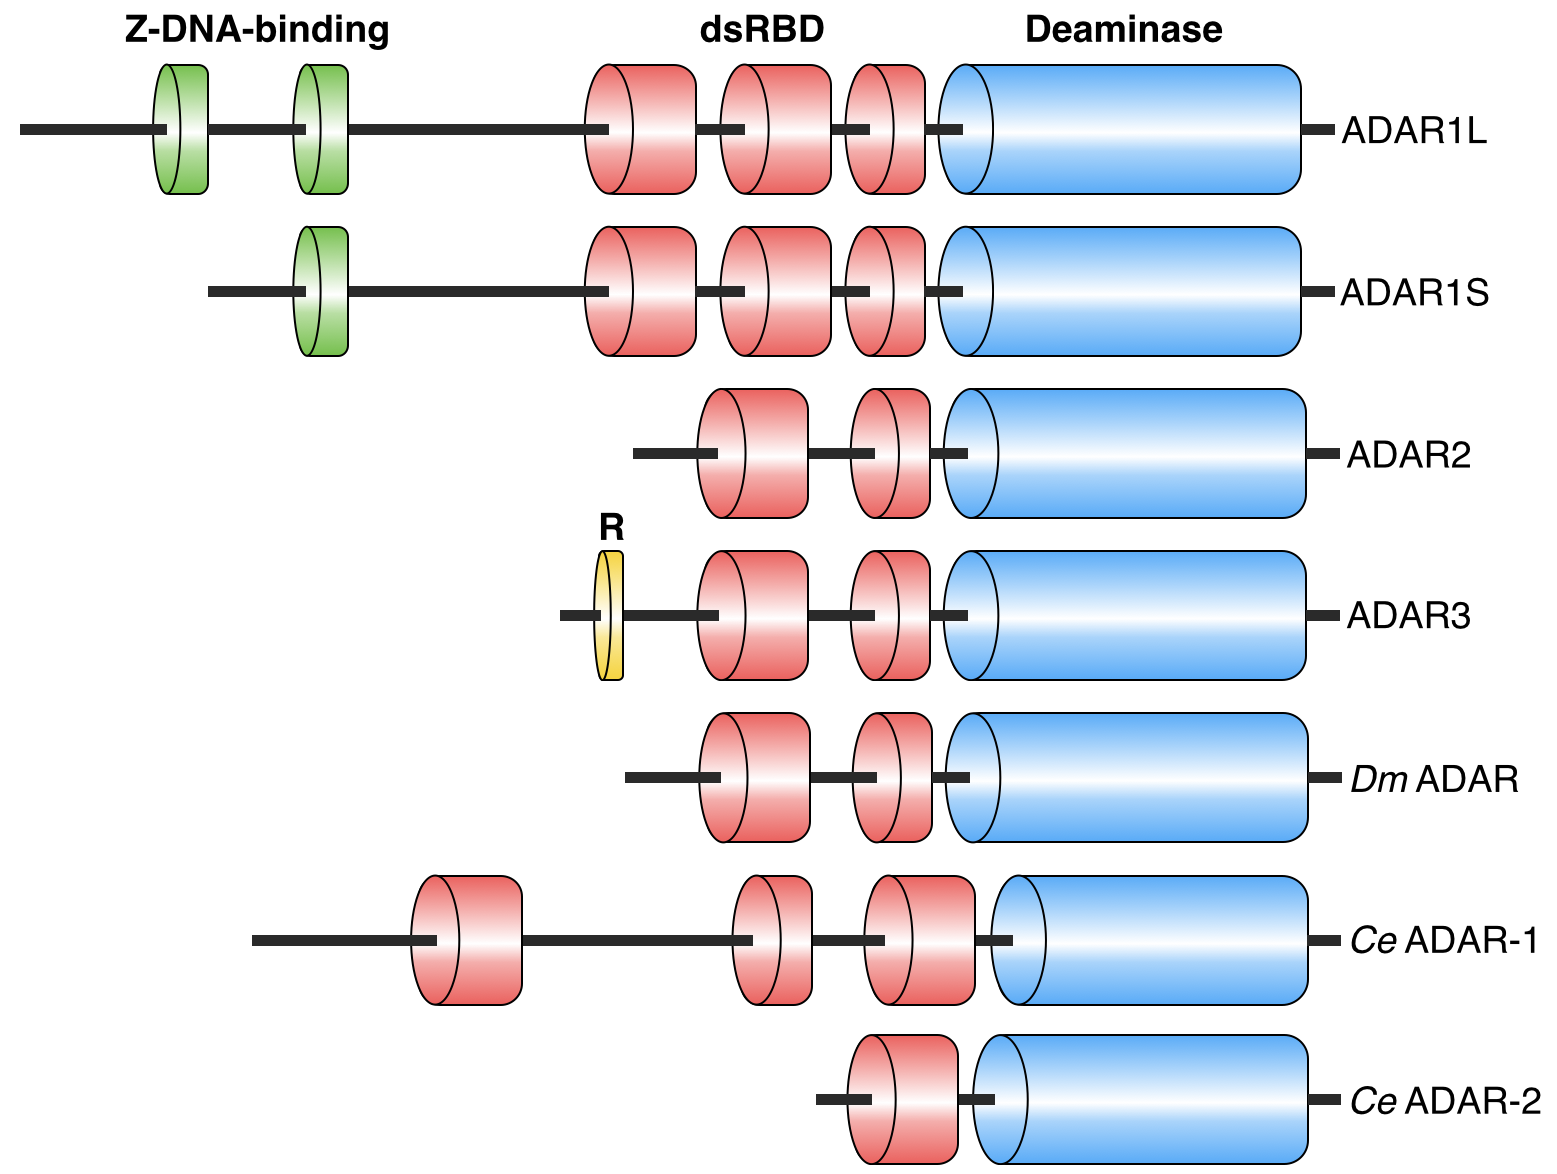
\includegraphics[width=11cm]{Adar_domain.png}
	\end{center}
	\caption{ADARのドメイン構造}
	\begin{flushleft}
		\small{ヒト、マウス、ショウジョウバエにおけるADARのドメイン構造を示す。左から順に、Z-binding (緑)、Double strand RNA binding (赤)、Deaminase (青)、Arginine-rich (黄)の通り、それぞれ機能ドメイン構造ごとに色分けして示した。}
	\end{flushleft}
	\label{fig:adar_domain}
\end{figure}

\subsection{ADARの発現と細胞内局在}
ADARは、核内おおよび細胞質のどちらにも局在することが知られる。ADAR1については核内および細胞質に局在するADAR1LおよびADAR1Sが知られる他、ADAR3は脳特異的に発現していることが知られる。核内で起こるA-to-I editingは、最近の研究によるとRNAポリメラーゼIIによる転写と同時、すなわちCo-transcriptionalに作用していることが主にショウジョウバエにおける核内の新生RNAを用いたトランスクリプトーム解析から報告されている。Co-transcriptinoalなA-to-I editingは、転写やスプライシングの効率に影響を与えているデータも示されており、ADAR1およびADAR2の細胞内局在とスプライシング機構との関係性については、今後より詳細が明らかにされるだろう。
\par
\textit{in vivo}においては、ADAR1およびADAR2はホモダイマーの形成が脱アミノ化には必須であることが報告されている。ADAR1は、インターフェロン誘導性のプロモーターによって転写が行われ、ADAR2の発現は、CREB (Cyclic adenosine monophosphate response element binding protein)による制御を受けていることが分かっている。
\par
また、ADAR2はself-editingと呼ばれる機構が知られており、発現しているADAR2のmRNAに対して数カ所のA-to-I editingを起こす。結果として、ADAR2-mRNAは4番イントロンと5番エクソンとの間に47塩基が挿入されたフレームシフト変異を引き起こし、新しいスプライスバリアントはediting活性を持たないことが報告されている。このことは、ADAR2が自身の活性をA-to-I editingにより制御するという非常に興味深い現象である。

\subsection{A-to-I editingの進化的な起源}
ADAR1およびADAR2は、真核生物における昆虫やイカ、脊椎動物など進化的に広く分布し、また高い配列保存性を示す。酵母や原生生物、植物においては発見されていない。ヒトにおいては、これまでにADAR1、ADAR2、ADAR3の3種類が同定されている。このうち、ADAR1およびADAR2は酵素活性が確かめられているが、ADAR3に関しては機能ドメインは保存されているが酵素活性については不明である。このADAR3は、脊椎動物のADAR2の遺伝子重複により生じたとも考えられている。
\par
加えて、Adenosine deaminase acting on tRNA (ADAT)と呼ばれるADARのタンパクファミリーが同定されており、ADATはtRNAのアンチコドンあるいはその近傍の塩基にA-to-I editingを起こす。ADATはヒトから酵母まで真核生物において広く保存され、バクテリアでもオーソログ遺伝子が同定されている。このことから、アデノシンからイノシンへの修飾をするタイプは、原核生物から真核生物まで広く存在しており、ADATはADARの祖先である可能性が示唆されている。
\par
A-to-I editingによる塩基修飾は、現存する生物が進化的な祖先種の遺伝子配列を獲得する復帰突然変異としての役割があるという仮説が提唱されている。筆者は、ヒト、チンパンジー、アカゲザルのゲノム配列から祖先種のゲノムを推定した。ヒトゲノムと推定した祖先種ゲノムとを塩基配列を比較すると、ヒトの90\%以上のA-to-G editingサイト (=グアニン)は祖先種においてもグアニンであった。このことは、進化の過程でアデニンへの一塩基置換が起こり再びその箇所をA-to-G editingすることで、祖先配列を獲得している可能性がある。このようなA-to-G editingにおける復帰突然変異のような現象を筆者はRNA memory仮説として提唱している。しかしながら、祖先種のゲノム配列を検証することは難しく、RNA memoryが何らかの制御を受けた結果であるのかは議論の余地が残されている。

\section{A-to-I editingの持つ多様な生理学的機能}
\subsection{タンパク機能の調節と多様化}
真核生物におけるRNA editingの重要な役割として古くから認識されてきたものは、コード領域内におけるアミノ酸配列の変化を伴ったA-to-I editingである。AMPA型グルタミン酸受容体は、GluR2サブユニットは他のサブユニットに対して膜上のアミノ酸がグルタミン (Q)から陽電荷を有するグリシン (R)へと変化しており、その結果としてGluR2サブユニットを有するAMPA型グルタミン酸受容体のみカルシウムに対して非透過性を示す。このカルシウム透過性に関する制御はQ/R調節とも呼ばれ、A-to-I editingによるグルタミン (CAG, Q)からグリシン (CIG, Q)への非同義置換によって達成されている。哺乳類の神経細胞においては、100\%に近い割合でQ/R調節が行われており、RNA editing率の低下は細胞内へのカルシウムの透過率をさせ、結果として細胞死やヒトの場合は疾患の原因となることが報告されている。
\par
5HT$_{2C}$RにおけるGタンパクとのカップリングサイト、AからEサイトのイノシン (AUA, I)からアスパラギン (AAU, A)への置換が起こる。5-HTの効力とリガンドとの結合親和性に影響する。
\par
タコの$K_{V}$チャネルには、14箇所のeditingが起こることが発見されている。このeditingを受けた$K_{V}1.1$チャネルは、非活性化へ影響する。

\textit{Drosophila}$K_{V}1.1$ カルシウムイオンチャネル、mammalian GABA receptor 3α、 dADARのself-editing siteなど。

\subsection{非コードRNAへのA-to-I editing}
これまでは、GluR2やKVチャネルなどコード領域の特定のグアノシンを選択的にイノシンへ置換することによるA-to-I editingの生理学的な影響を概観してきた。ところが前述したとおり、EST (Expression Sequence Tags)配列や超並列シーケンサーによるA-to-I editingの網羅的な観察が可能になると、LINEやSINE、Alu配列などの反復配列、またUTRやイントロンなどノンコーディング領域におけるeditingが全体の80\%程度を占めるということが明らかとなった。こうった背景から、遺伝子領域をターゲットとしたA-to-I editingから反復配列やノンコーディングRNAとA-to-I editingの関係性についての解析が一挙に推し進められるようになった。
\par
興味深いことに、A-to-I editingは、核内外においてDicerやDrosha、RISCなどRNA結合タンパク複合体や、miRNAやepiRNAなど他のRNAと相互作用を起こすことが明らかとなってきた。こういった現象は、A-to-I editingがタンパク質の機能を多様化させる他にも、真核生物はノンコーディング領域におけるA-to-I editingを介して積極的な遺伝子発現制御を行う可能性を示唆するものである。

\subsection{二本鎖RNAの安定性への寄与}
ADARによるA-to-I editingは、二本鎖RNAが形成する折りたたみ構造に依存し、

RNA分子における塩基対形成は、I:UおよびG:Cのワトソン・クリック型塩基対を安定的に形成するが、A-to-I editingにより一般的なワトソン・クリック型塩基対ではなく、I:Uがペアリングするゆらぎ塩基対 (Wobble base pair)を形成する。このゆらぎ塩基対は、二本鎖RNAを熱力学的に不安定化させる。またこの逆に、A:Cなどのゆらき塩基対に対するA-to-I editingは、二本鎖RNAの安定化に寄与すると考えられる。このように、A-to-I editingによる塩基対形成の変化は、局所的または大域的に二本鎖RNAの安定性を変化させると考えられている。

%\subsection{ヘテロクロマチンを介した遺伝子サイレンシング}

\subsection{スプライシング機構との関連性}
真核生物のほぼ全てのエクソン-イントロン境界は、GU-AG配列と呼ばれる強いコンセンサス配列が保存されており、スプライシング機構においてイントロン配列の切り出し位置が決定されている。5' splice siteはacceptor site、3'はdonnar siteと呼ばれ、AU配列またはAG配列へのA-to-I editingはそれぞれ新生のacceptor site、donnar siteを形成する。また、AG配列へのA-to-I editingは、3' splice siteを欠失することがこれまでに報告されている。また、このようなsplice siteの新生や欠失が二本鎖を形成したAlu配列に起こる場合、Alu配列の一部がエクソン化し、成熟mRNAに新たなエクソンとして取り込まれる例がヒトのNuclear prelamin A recognition factor (NARF)タンパクでは知られている。このようなA-to-I editingによるAlu配列のエクソン化は、新たな機能を持つタンパク質のバリアントを生み出すため、進化的に重要な役割を担っていると考えられている。
\begin{figure}[!htbp]
	\begin{center}
		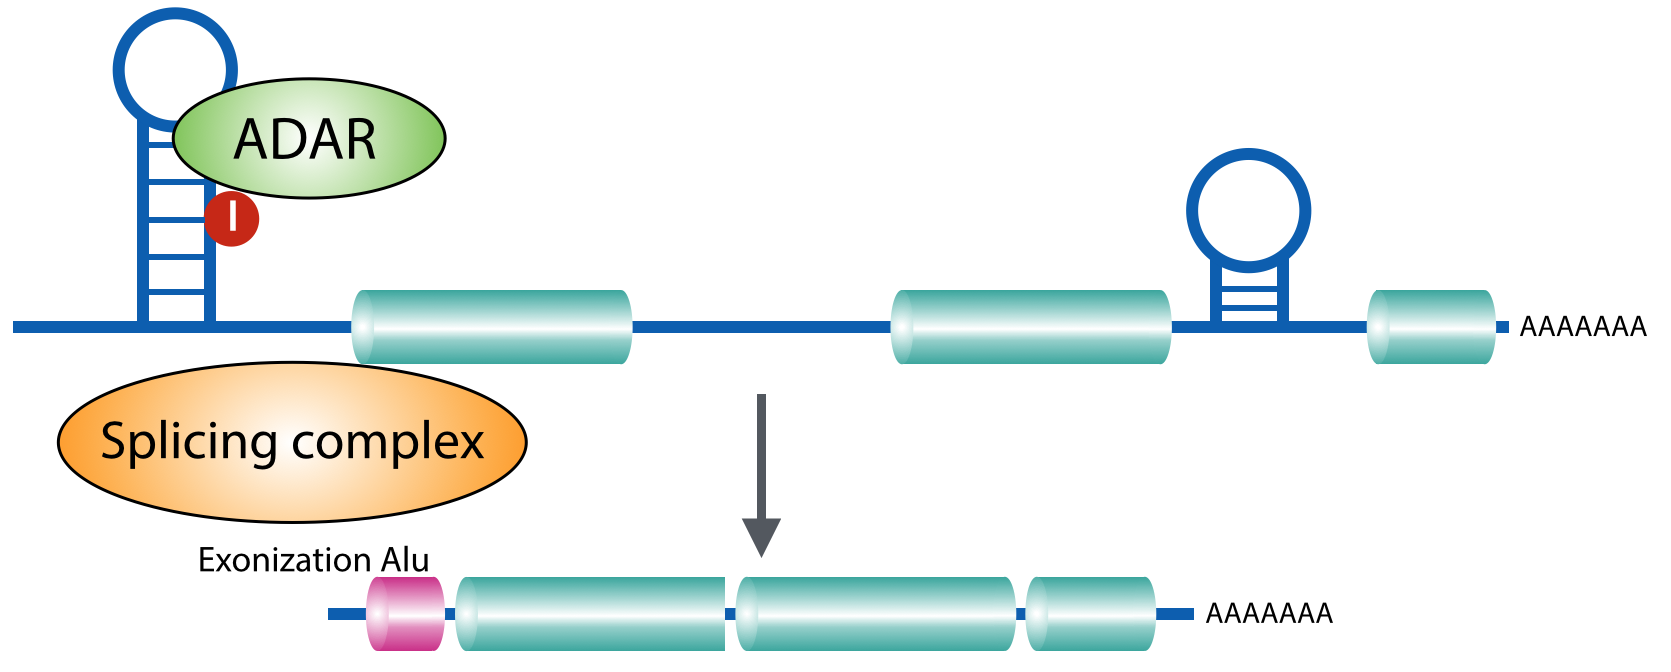
\includegraphics[width=14cm]{Alu_adar.png}
	\end{center}
	\caption{Alu領域へのA-to-I editingによるエクソン化}
	\begin{flushleft}
		\small{二本鎖RNAを形成したAlu領域において、A-to-I editingが入るとAluの一部が新生のエクソンとしてスプライシング機構によりエクソン化し、翻訳される。}
	\end{flushleft}
	\label{fig:Alu_adar}
\end{figure}

\subsection{miRNAへのA-to-I editingと遺伝子発現制御}
低分子RNA (Small RNA)の一種として知られるmiRNAは、複数のRNA結合タンパクと相互作用し、転写されたmRNAに対して分解を促進し、遺伝子の翻訳抑制を行う
真核生物において重要な低分子RNAの一つである。miRNAは、初めは数百から数千塩基程度のpri-miRNA (primary-miRNA)として転写されDroshaとDGCR8が形成する複合体によりヘアピン構造のpre-miRNAとして切り出され、細胞質へ輸送される。細胞質では、pre-miRNAはDicer-TRBP複合体による切断を受けた後に、21塩基程度の二本鎖RNAとなり成熟する。miRNAは、RISC (RNA-induced silencing complex)へと取り込まれ、標的となった遺伝子の3'末端の非翻訳領域に結合し、mRNAの分解に作用する。
\par
pri-miRNAからmiRNAへと成熟する過程では、二本鎖RNAを形成するためDroshaやDicerによる切断と同様にADARによるA-to-I editingもその標的となる。

Dicerは、RNase IIIに属する二本鎖RNAを切断する。
Droshaは、
これまでに、miRNAの生合成経路におけるADARとの相互作用には、miRNAの産生を活性化および拮抗作用という相反する機序が報告されている。
このように、二量体を形成したADAR1-Dicer複合体は、miRNAに対するA-to-I editingは拮抗的に作用することが知られているが、近年ではmiRNA産生の活性化にもADARが関与していることが明らかとなってきた。
miRNA産生を活性化する際、Dicer-ADAR1複合体を形成しており、この二量体はeditingを起こせず、この

\begin{figure}[!htbp]
	\begin{center}
		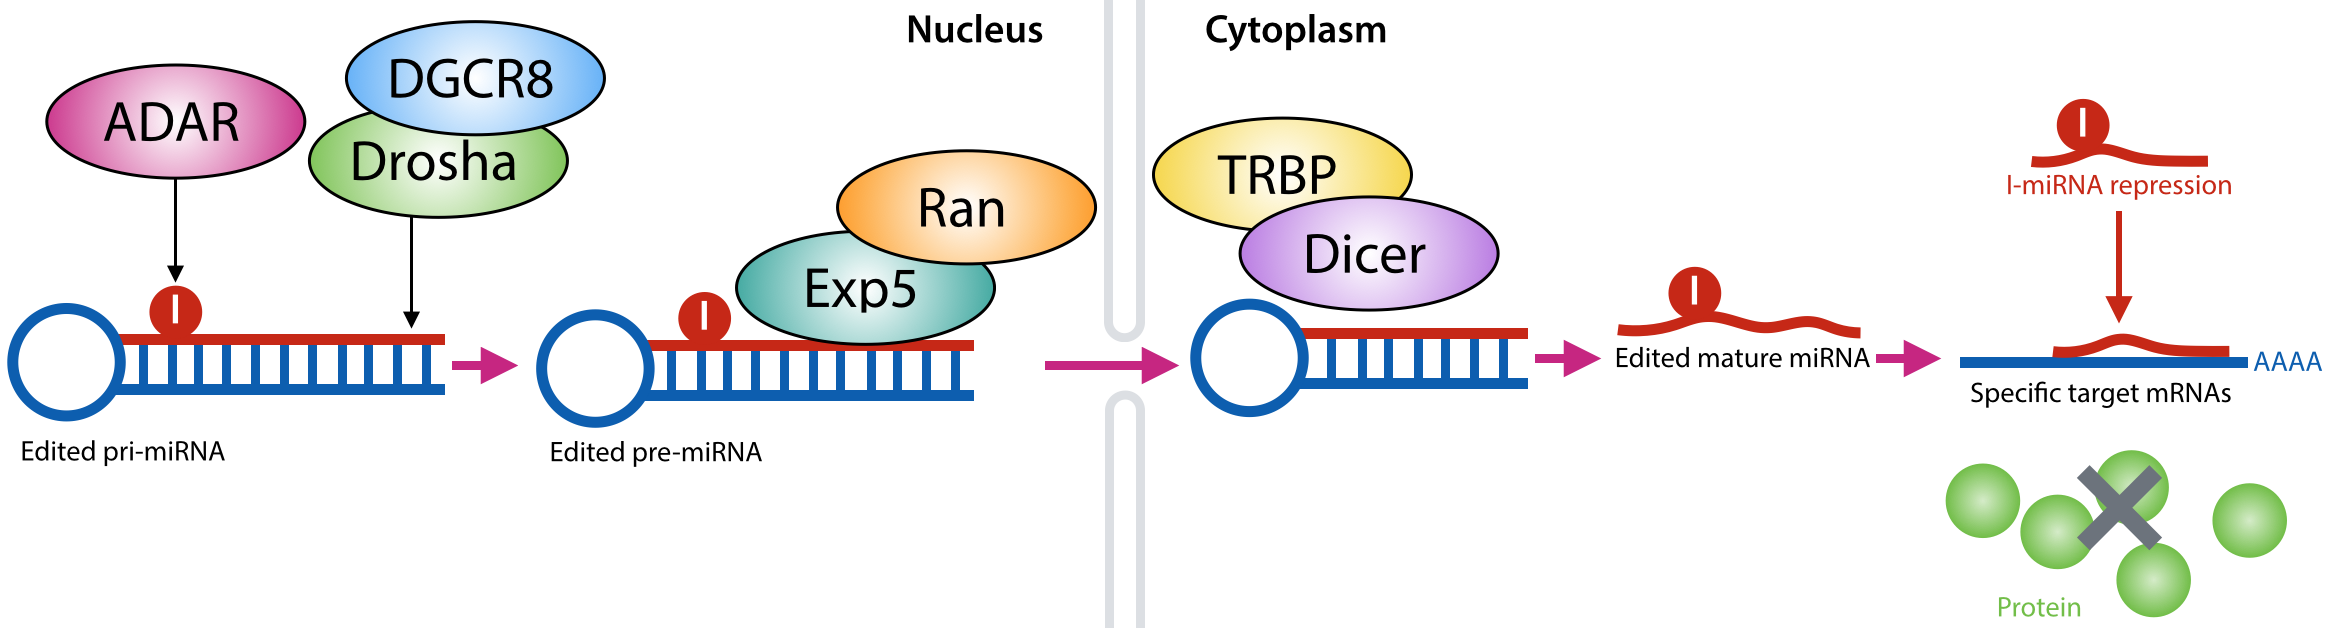
\includegraphics[width=16cm]{miRNA.png}
	\end{center}
	\caption{miRNAへのA-to-I editing}
	\begin{flushleft}
		\small{miRNAの成熟過程においてA-to-I editingを受ける。miRNAの成熟過程では、Drosha-DGCR2複合体やTRBP-Dicer複合体における切断部位へのA-to-I editingが知られており、それぞれは異なる応答を示す。転写されたpri-miRNAは、Drosha-DGCR2複合体による二本鎖RNAを標的として切断を受けpre-miRNAとしてRan-Exp5複合体により細胞質へと輸送される。細胞質ではTRBP-Dicerによる切断を受け、成熟したmiRNAとなる。}
	\end{flushleft}
	\label{fig:miRNA}
\end{figure}

\subsection{A-to-I editingによるsiRNA産生の制御}
miRNAの生合成過程におけるA-to-I editingと同様に、Dicerのよる切断を受けて成熟するsiRNA (small interfering RNA)もまたA-to-I editingの影響を受けていることが近年、明らかになりつつある。siRNAはDicerによって21から24塩基程度の二本鎖RNAへと切断され、miRNAと同様にRISCを形成する。RNAi経路においては、siRNAと相補的な配列を有する遺伝子が転写抑制の標的となるため、Argonauteタンパクなどの複合体としてRISCに取り込まれたsiRNAは標的遺伝子を認識する重要な役割を持つ。
\par
これまでsiRNAの産生は、ウィルスなど外来性RNAに由来すると考えられてきたが、マウスの卵母細胞を用いた実験では、SINEなどレトロトランスポゾンが形成する長鎖ヘアピン (lhRNA, long-hairpin dsRNA)二本鎖RNAがDicerの標的ととなって、内在性siRNA (endogenous si RNA)が生成する経路が報告された。この内在性siRNAは、トランスポゾン活性に対して抑制性に機能するsiRNAである。\textit{in vitro}の実験結果から、A-to-I editingを受けた内在性siRNAはDicerによる切断に対して抵抗性を示すことが分かった。これは、A-to-I editingによって、二本鎖RNAにおいてはA:IからA:Uへ塩基対形成が変化する。A:U塩基対は、Dicerの切断に対して抵抗性を示すため、A-to-I editingは内在性siRNAの産生量を減少させる、或いは正常に機能しない内在性siRNAの産生の制御にA-to-I editingが関与する可能性を示唆していると考えられる。

\begin{figure}[!htbp]
	\begin{center}
		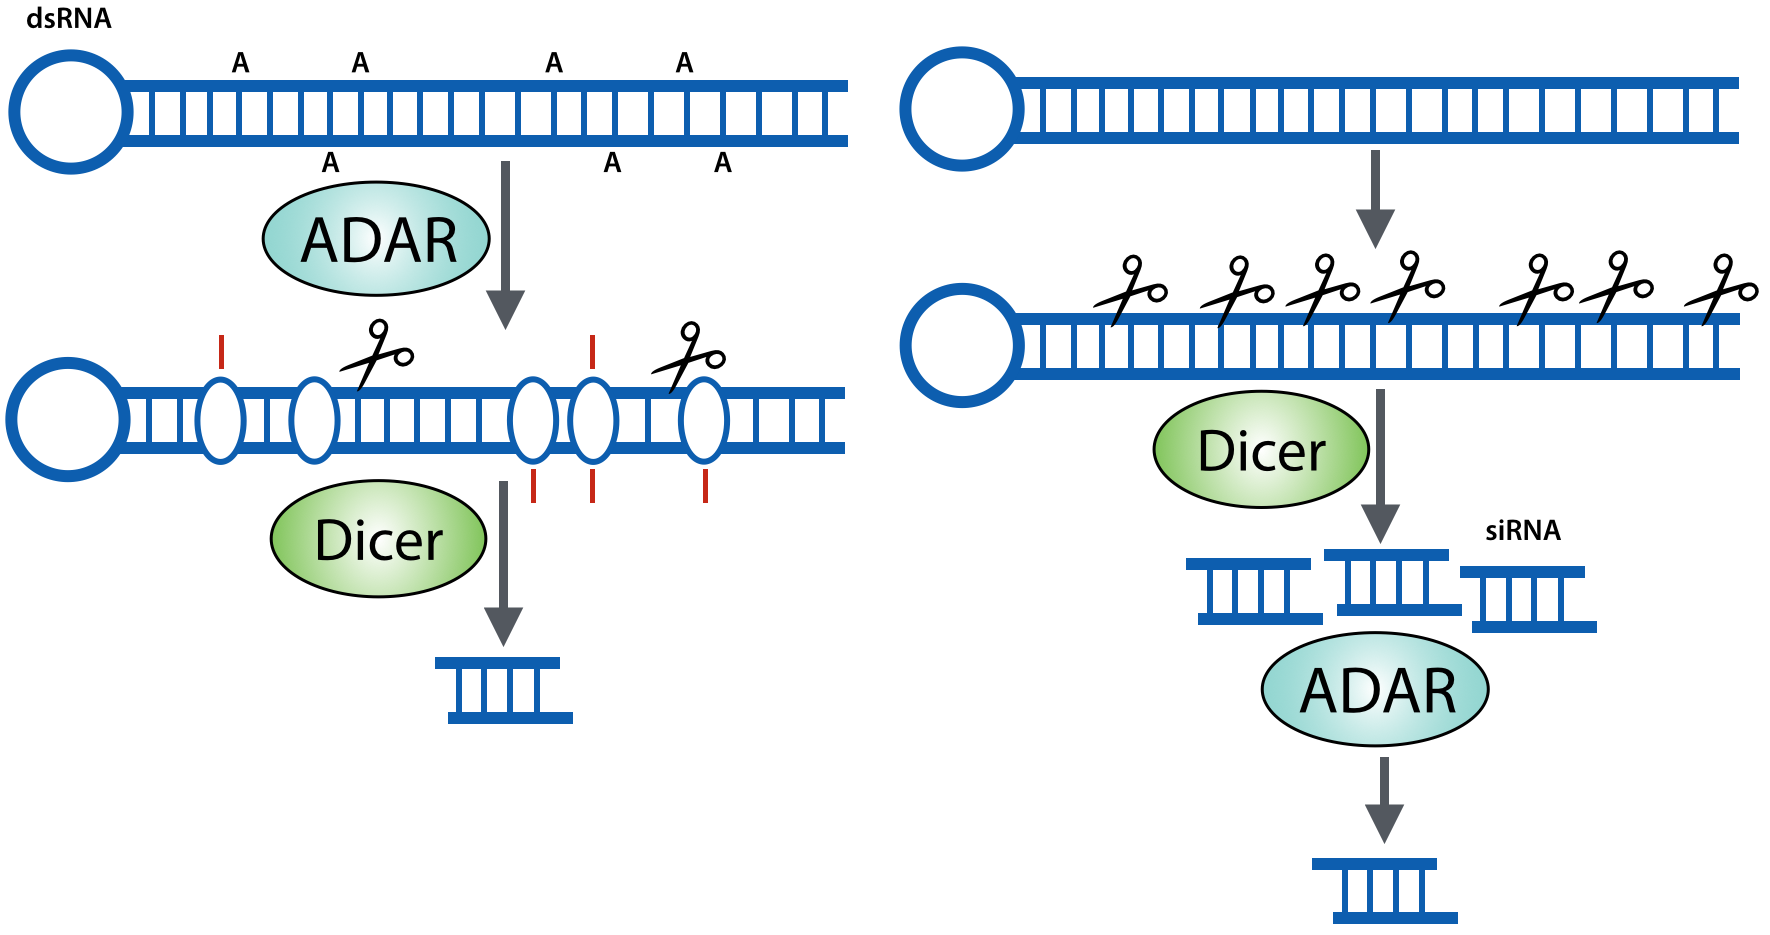
\includegraphics[width=14cm]{siRNA.png}
	\end{center}
	\caption{ADARによるsiRNAの制御}
	\begin{flushleft}
		\small{長鎖非翻訳RNAは、Dicerによる切断を受けて内在性siRNAとして機能する。現在考えられているA-to-I editingによるsiRNAの制御を左右にそれぞれ示した。左は、A-to-I editingを受けた長鎖ヘアピン二本鎖RNAへのがDicerへの切断抵抗性を示すために、内在性siRNAの産生量が減少する場合である。右は、既に生成されたsiRNAに対して、細胞質に局在するADAR1が強く結合することにより、siRNAのRISCへのローディングを阻害するし、siRNA濃度を減少させる場合である。}
	\end{flushleft}
	\label{fig:adar_siRNA}
\end{figure}

\subsection{A-to-I editingによるRNAiの制御}
線虫においては、二本鎖RNAがADARによるA-to-I editingを受けることによりRNAiへの経路を阻害することが報告されている。このように、RNAi経路に対して拮抗的に作用することが報告されている。
この拮抗的な作用とは真逆に、RNAi経路へ促進する機能も同時にADAR1は有していることが報告された。これは、ADARとDicerがホモ二量体の複合体を形成した場合であり、Dicer-ADAR1複合体はA-to-I editing能を持たない。

\section{情報学的解析によるRNA editingサイトの検出}
\subsection{超並列シーケンサーを用いた網羅的解析}
ここ数年、超並列シーケンサーに代表される配列決定技術の躍進的な発展は、多サンプルのゲノムおよびトランスクリプトームのシーケンスを可能にしてきた。RNA editing研究においては、超並列シーケンサーから得られるRNA-seqデータやDNA-seqデータを用いることにより、網羅的で定量性のあるeditingサイトを検出する情報学的手法が精力的に開発されている。超並列シーケンサーから測定されるトランスクリプトームやゲノムの配列情報は、数GBから数百GBの配列データを扱うことになるため、editingサイトの検出は本質的に情報学的な解析が必須となっている。2009年にLiらは、初めてヒトB細胞のRNA-seqデータを用いることにより、10,000箇所を超えるeditingサイトがゲノムワイドに同定されたと報告した。検出された修飾のパタンは、ADARによるA-to-I editing以外にも、A-to-T editingなど未知の修飾の可能性が残されていることを示唆する議論を展開した。また、同定されたeditingサイトは遺伝子間領域にも豊富に分布していること、アミノ酸置換を伴うeditingサイトを新規に同定したと報告した。ところが、この研究が掲載された後、3つの解析結果に対する追従論文が発表され、Liらによる解析結果の95\%以上は擬陽性の可能性があること、解析における擬陽性の原因と排除するための統計的な手法についての提案がされた。

こういったRNA-seqデータを用いることによるゲノムワイドなeditingサイトの分布が明らかになるにつれて、ヒトやマウス、ショウジョウバエといった高等真核生物におけるRNA editingの作用機序、生体内における機能そのものを大きく拡張することになった。
タンパク質の触媒部位へ作用することにより、
\par
超並列シーケンサーを用いたトランスクリプトーム解析が容易となった今日において、RNA editingサイトをRNA-seqデータを用いた研究はここ数年で大きく発展している。超並列シーケンサーから得られるRNAの配列は、転写物の発現量定量には十分の精度であると言えるが、一塩基の変異を正確に検出することが求められるRNA editingサイトの検出においてはその限りでなく、真のeditingサイトとエラーサイトを高精度に分離することが求められる。前述した通り、RNA editingサイトの検出には、cDNAを作成するための逆転写酵素の活性とそれに付随するPCR反応の増幅バイアス、RNA分子の不安定性など実験デザインが塩基決定に及ぼす影響、得られた配列の参照ゲノム配列へのマッピングとそのパラメータといった下流の解析デザインなどが多数のパラメータを最適化する必
要がある。

\subsection{ノイズのフィルタリング手法}
Liの研究、一連の研究のコメントなど。
各種バイアスの同定とフィルタリング方法について。

\subsection{トランスクリプトームワイドな傾向解析による知見}
マウスのeditingは、3'UTRにエンリッチする

\subsection{組織およびセルライン特異的なA-to-I editing}
ヒトの8つのセルラインを用いて、核内と細胞質を分離したRNA-seq解析からは、核内で起こるA-to-I editingが細胞質で起こるものより数倍以上高頻度である傾向が見られることから、A-to-I editingの多くはCo-transcriptionalに起きていることを示唆していると考えられる。核内と細胞質ともに70\%がセルライン特異的なA-to-I editingを占めることが報告されている。

